\chapter{Use Cases}
\label{sec:usecases}
In this chapter, we show how \msname can be used in applications and describe how it can solve the problems presented in Section~\ref{sec:problem}.

\section{Avoiding Duplicate Class Names}
\begin{wrapfigure}{l}{0.55\textwidth}
	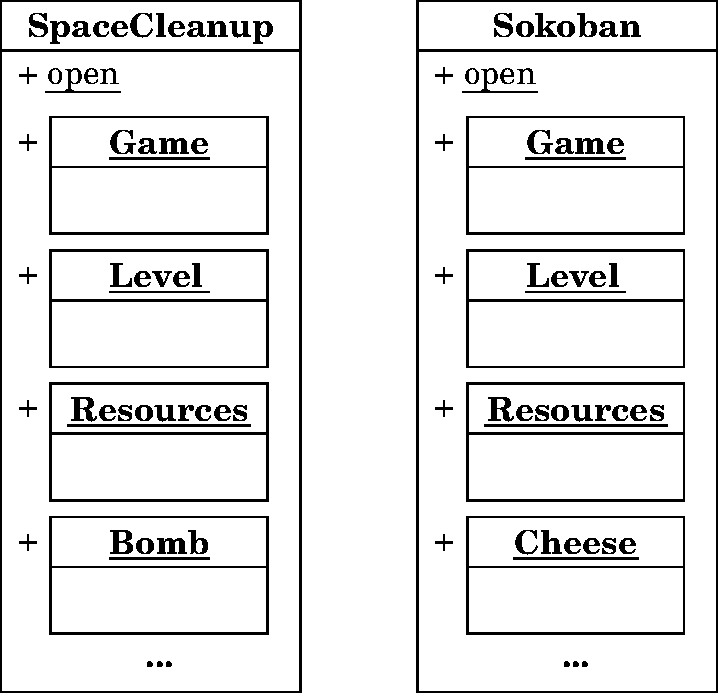
\includegraphics[width=0.5\textwidth]{usecase_class_clash.pdf}
	\centering
	\caption[Example: Avoiding duplicate class names]{Example: Avoiding duplicate class names. Every nested class has a unique fully qualified name.}
	\label{fig:use_class_clash}
\end{wrapfigure}

In this example, class nesting is used to avoid class name clashes and to give every class a unique fully qualified name. Consider, that we want two load two computer games in a single Squeak image. The first game is a bomberman game (SpaceCleanup), providing classes \texttt{Game}, \texttt{Level}, \texttt{Resources} among others. The second game is a Sokoban game, and has three classes with the same name. Without \msname, this would be a problem: as soon as another class with the same name is installed, the old one is overwritten with the new one.

With \msname, two classes with the same name can coexist in the same image, as long as they are nested within different classes (Figure~\ref{fig:use_class_clash}).

Note, that, for example, \texttt{SpaceCleanup Game} and \texttt{Sokoban Game} are different classes. Whenever a class inside \texttt{SpaceCleanup} references \texttt{Game} using the source code statement \texttt{scope Game} or \texttt{Game} (equivalent statements), the method lookup recurses in the enclosing class, until \texttt{Game} is found in the \texttt{SpaceCleanup} class.

\section{Module Versioning and Dependency Management}
In this example, class nested is used to keep multiple different versions of the same library in one image. This is necessary if two applications require different versions of the same library. In the best case, the API of a library should not change within one major version, such that a newer library version should work with an application that was developed with an older library version. However, sometimes, application developers have to work around known bugs or rely on implementation-specific classes which are not designed to be used by library users and subject to change. In that case, application code can break when suddenly a different version of the library is used.

\subsection{Representing Module Versions}
\begin{wrapfigure}{l}{0.55\textwidth}
	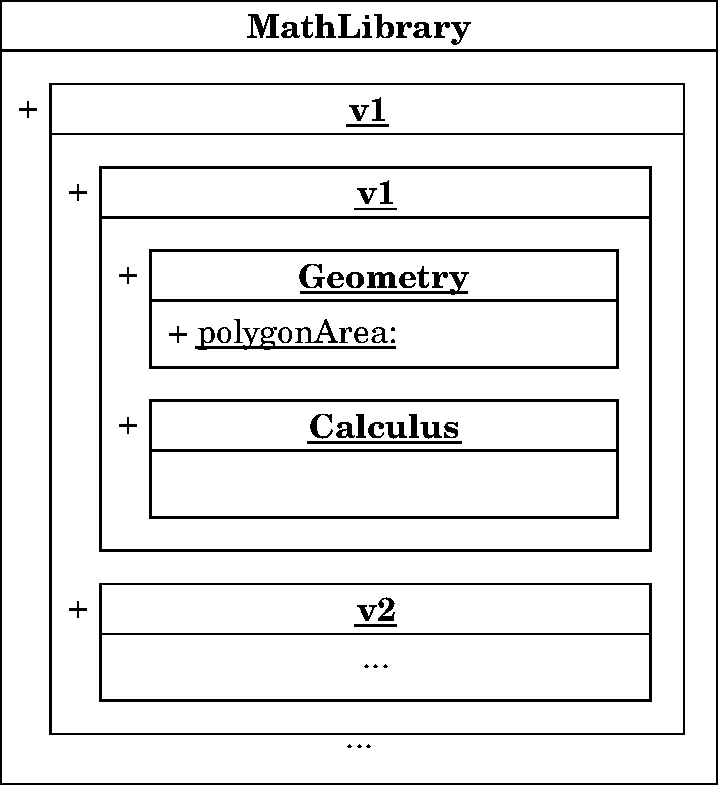
\includegraphics[width=0.5\textwidth]{usecase_define_version.pdf}
	\centering
	\caption[Example: Module versioning]{Example: Module versioning. A version is represented by a nested class.}
	\label{fig:use_module_ver}
\end{wrapfigure}

Figure~\ref{fig:use_module_ver} shows how nested classes can be used for module versioning. In this example, we are developing a library for mathematical operations. The top-level class contains nested classes for every major version. Every major version can again have nested classes for minor versioning. In fact, this scheme can be used to have any kind of versioning system, as long as it is based on numbers.

Two versions of \texttt{MathLibrary} are installed in this example: version 1.1 and version 1.2. These versions can be referenced by writing \texttt{MathLibrary v1 v1} and \texttt{MathLibrary v1 v2}. Note, that even though all versions define classes with the same name, no class clashes occur. If a class in \texttt{MathLibrary} references another class in \texttt{MathLibrary}, the method lookup will look for classes in the same version of \texttt{MathLibrary}.

\paragraph{New Versions}
In case the programmer wants to add a new version, \msname will in future releases provide a mechanism to copy a base version and give it a new name. The copied base version can then be modified. Already released versions should not be changed in the future. Instead, a new version should be released.

For development purposes, it is useful to have a special version called \texttt{dev}. Programmers can collaboratively work on this version. Once the version should be released, the programmer can make a copy of the entire class and give it a new name: the new version number.

\msname does at the moment not support delta updates. A new version is always an entire copy of an application, even if just a few methods changed. We might consider delta updates in future releases of \msname, such that a new version is essentially the previous version and a set of changed methods/classes. Of course, this requires having the entire application history installed in the image.

\subsection{Aliasing Module Versions}
Whenever an application requires a class from a library in a certain version, the application can either write down the fully qualified name of the class or create an alias. For example, the fully qualified name of the class \texttt{Calculus} in \texttt{MathLibrary} version 1.2 is \texttt{MathLibrary v1 v2 Calculus}. However, it is very likely that an application requires more than just one class from a library. In this case, an alias should be defined, because it keeps the required version number at a single point in the code (making it easy to change the version) and results in less verbose code.

\begin{figure}[!htp]
\begin{lstlisting}
<@\textbf{MyApplication>>MathLibrary}@>
    ^ Repository MathLibrary v1 v2

<@\textbf{MyApplication>>rectArea:}@> origin <@\textbf{extent:}@> extent
    ^ MathLibrary polygonArea: { 
        origin x @ origin y.
        (origin x + extent x) @ y.
        (origin x + extent x) @ (origin y + extent y).
        origin x @ (origin y + extent y) }
\end{lstlisting}
\caption{Defining class aliases}
\label{fig:use_alias}
\end{figure}

Figure~\ref{fig:use_alias} shows how class aliases can be used to specify module versions at a single point in the code. The programmers defines a method \texttt{MathLibrary} returning the module in the required version. In \texttt{MyApplication>>rectArea:extent:}, the reference to \texttt{MathLibrary} will be replaced with \texttt{scope MathLibrary}, which will call the aliased method. Note, that in \texttt{MyApplication>>MathLibrary}, we have to reference the library with \texttt{Repository MathLibrary}, forcing the lookup to start at the root of our system. Otherwise, the method \texttt{MathLibrary} would call itself.

Classes aliases, as described in this paragraph, are similar to import statements in other programming languages, and are a form of internal dependency management.

\paragraph{Helper Methods}
In Figure~\ref{fig:use_module_ver}, the top-level class and major version should be a subclass of the class \texttt{Versioning}, a class provided by our system. This class contains convenience methods making it easier to work with version containers. The following list gives an overview of the helper methods \texttt{Versioning} provides.

\begin{itemize}
	\item \texttt{Versioning>>myLatest}: returns the latest version contained as a nested class in the receiver. For example, \texttt{MathLibrary myLatest} returns \texttt{MathLibrary v1}.
	\item \texttt{Versioning>>latest}: returns the lastest version in the receiver recursively. For example, \texttt{MathLibrary latest} returns \texttt{MathLibrary v1 v2}.
	\item \texttt{Versioning>>atLeast:}: returns the latest version recursively and asserts that its version number is greater than the parameter. For example, \texttt{MathLibrary atLeast: '1.1'} returns \texttt{MathLibrary v1 v2}, and \texttt{MathLibrary atLeast: '1.3'} throws an error.
\end{itemize}

In order to get the latest installed version with major version \texttt{1}, the programmer could write \texttt{MathLibrary v1 latest}. Future versions of \msname might automatically download and install missing versions, instead of throwing an error message.

\subsection{Squeak Versioning}
With \msname, it is theoretically possible to run multiple versions of Squeak in one image. The basic idea is that every Squeak version is nested in a different version class. The screenshot in Figure~\ref{fig:usecase_browsers} shows two versions of the system browser running in the same image. The old system browser lacks many features, such as syntax highlighting or buttons for senders/implementors.

\begin{figure}[!htp]
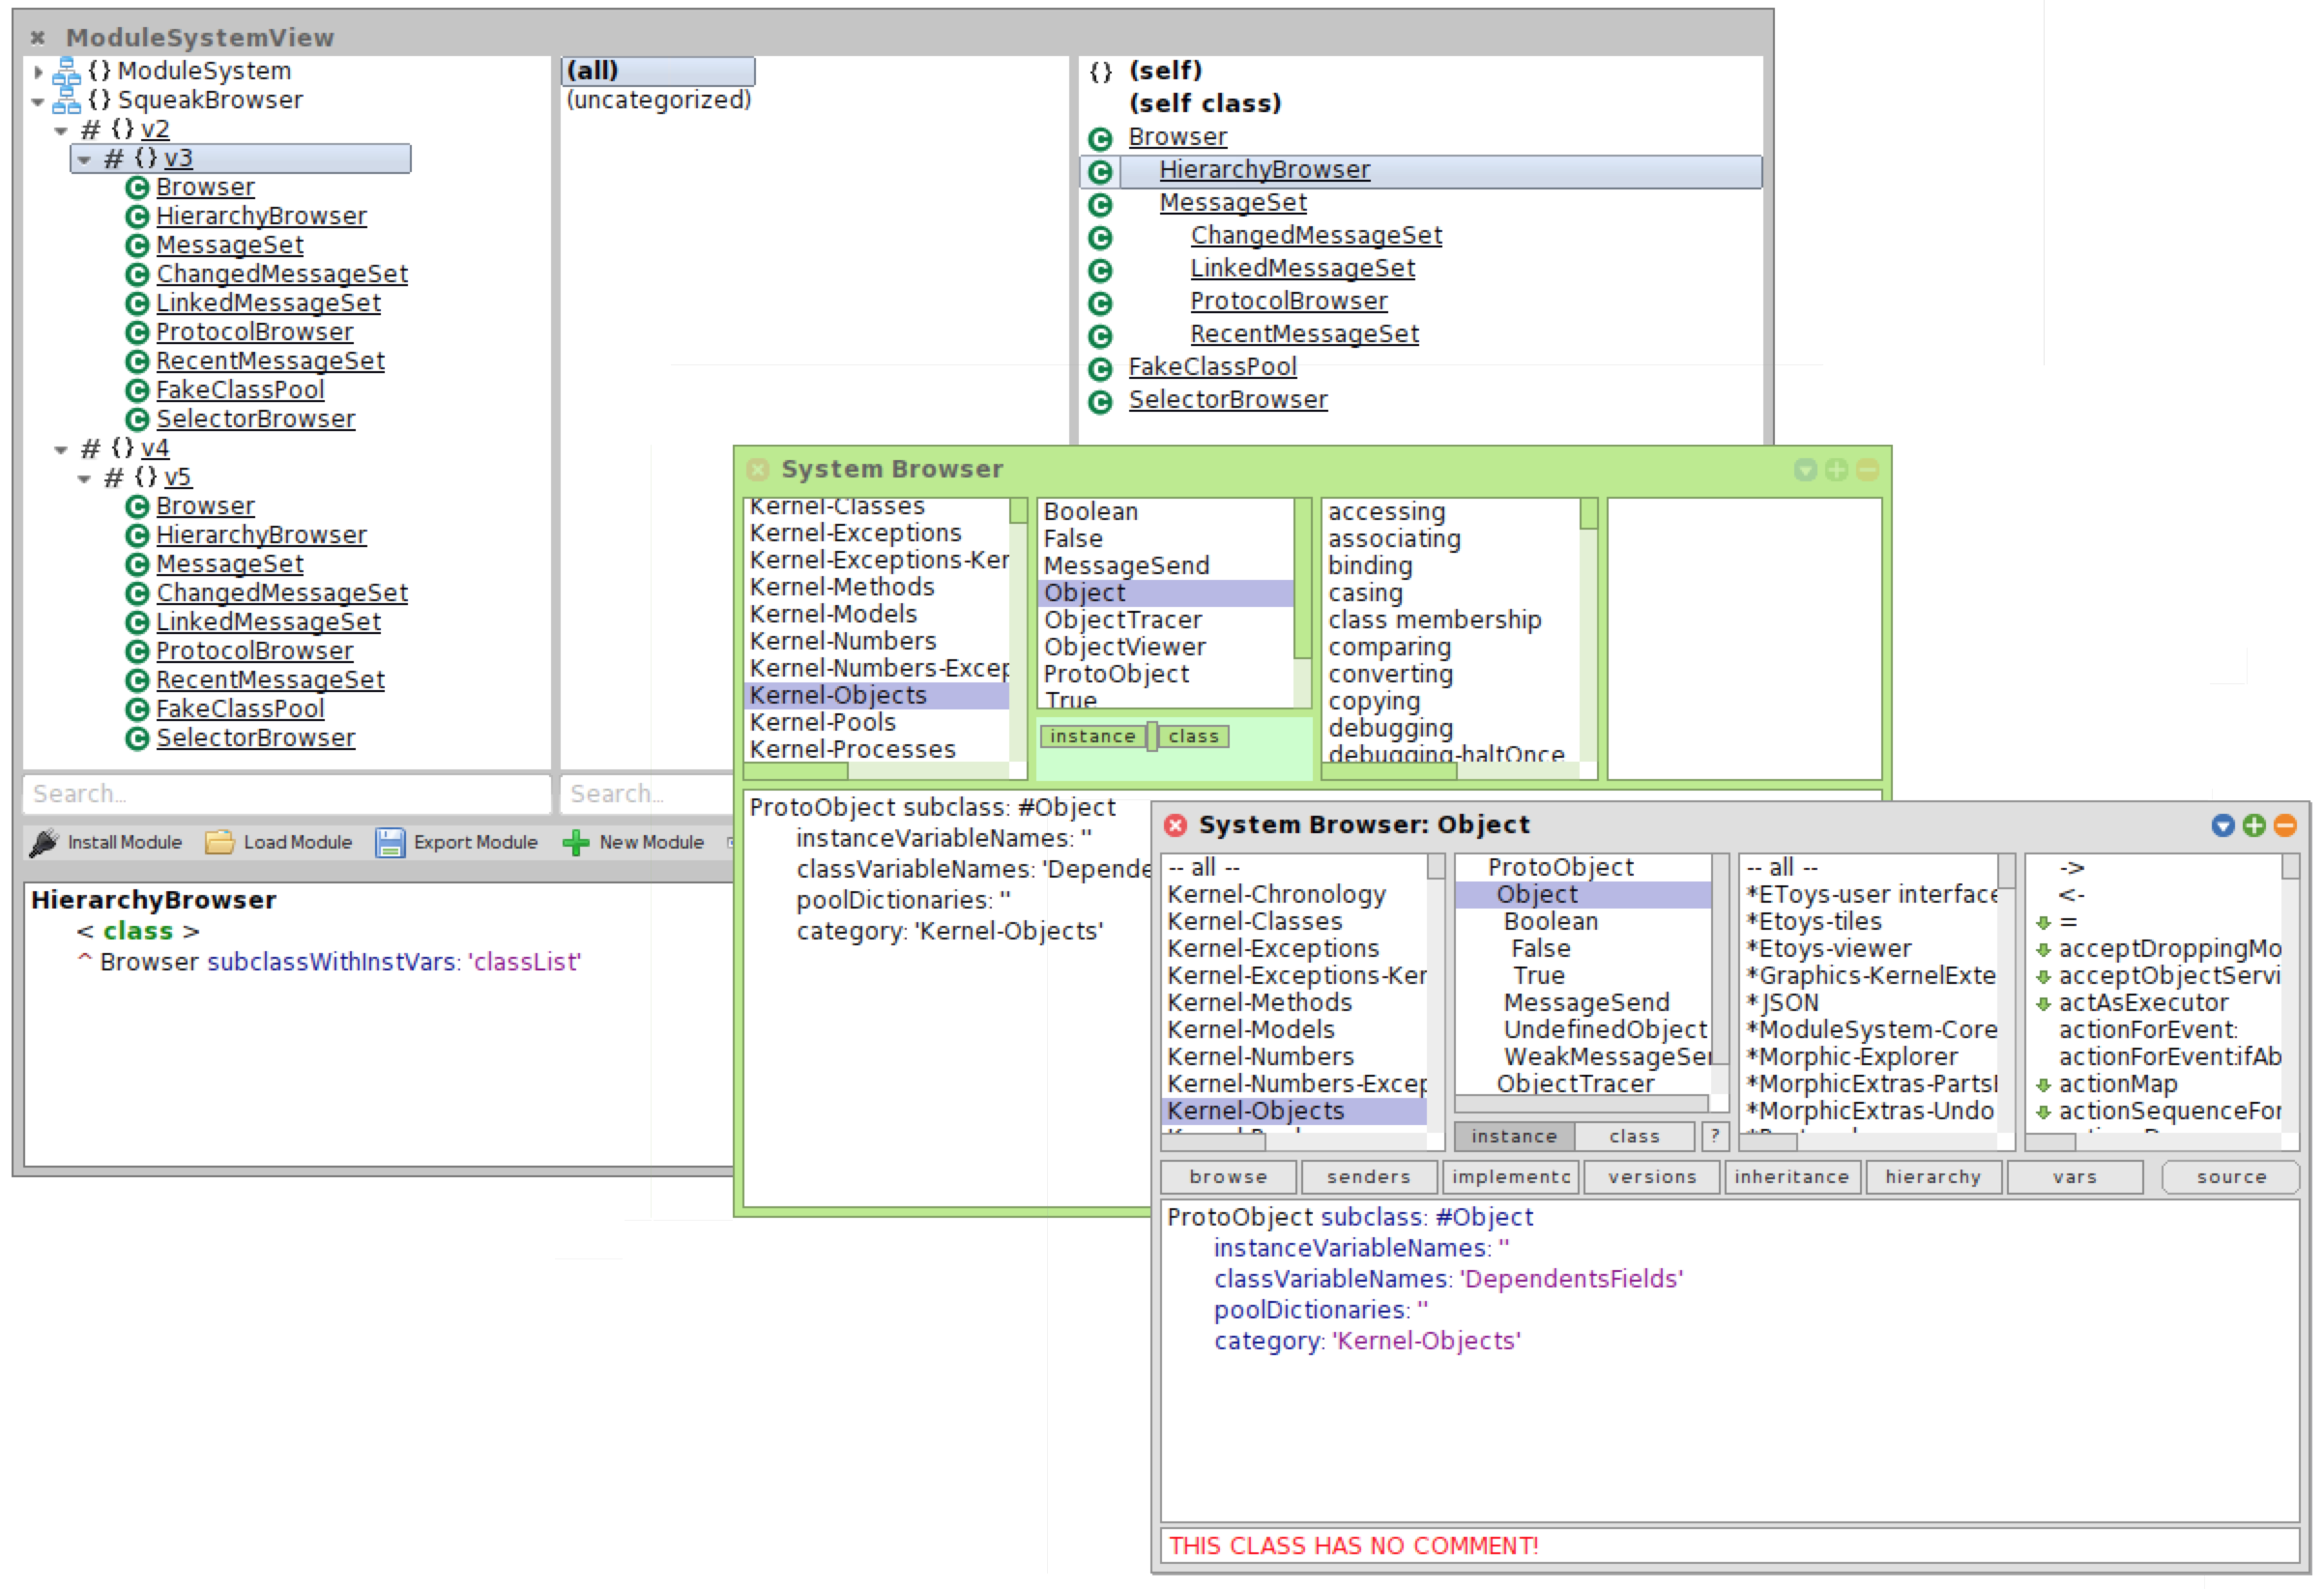
\includegraphics[width=\textwidth]{usecase_browsers.png}
\centering
\caption[Example: Squeak system browser in different versions]{Example: Squeak system browser in different versions. The browser in the front is a modern Squeak~4.5 system browser. The browser in the back is a system browser from Squeak~2.3.}
\label{fig:usecase_browsers}
\end{figure}

When we tried running bigger system libraries, such as Morphic, in different versions in one image, we encountered the following difficulties.
\begin{itemize}
    \item Many system libraries are not written in a modular way. For example, they use global state. Whenever global state is stored on other classes or in the \texttt{globals} dictionary (e.g. \texttt{Smalltalk globals at: \#World}), the library circumvents \msname.
    \item Some classes should not exist multiple times in one image. For example, \texttt{Array} and \texttt{String} are classes that the virtual machine knows about\footnote{\texttt{SmalltalkImage>>specialObjectsArray} calls primitive 129 and returns an array of 56 unique special objects that the VM knows about.}. Whenever an argument is passed to a primitive, the virtual machine expects that it is an instance of a class it knows about. Similarly, whenever a primitive returns a value, it is an instance of the version the image knows about.
\end{itemize}

Future work might investigate how multiple Squeak versions can be run in a single image.

\subsection{External Configuration}
Parameterized classes can not only be used to build mixins, but also externally configuarable modules. The basic idea is taken from Newspeak, where all module dependencies are encapsulated in a \texttt{platform} object. This platform object is installed along with the application source code and contains all libraries that the application depends on in the correct version~\cite{bracha2008newspeak}. This has the advantage that there is no need for a global namespace and all references to external classes are resolved using the platform object, effectively making import statements obsolete. A configurable module does not need to know anything about concrete implementations of external libraries, as long as the implementations provided in the platform implement the expected interfaces.

In our system, methods inside parameterized classes can reference arguments provided to the class accessor method. The idea is that, instead of referencing classes in the global namespace, the programmer references these arguments. The user of the module can then decide which exact implementation he wants to use.

\paragraph{Example}
Figure~\ref{fig:use_paintbrush} shows part of the implementation of a simple drawing application. \texttt{PaintbrushWith:IO:} is a parameterized top-level class which takes as arguments a matrix implementation and a file IO library. The matrix implementation is used for storing the pixels inside the application. In the simplest case, this could be the class \texttt{Matrix} from the Squeak standard library. It could, however, also be a class which stores pixels in a compressed form (e.g., using run-length encoding), but has \texttt{at:}, \texttt{at:put:}, \texttt{rows}, and \texttt{columns} as public API methods. \texttt{ReaderWriter} must be a class or object that supports reading and writing files on a pixel-by-pixel basis. Depending on which IO class the user of the library provides to \texttt{PaintbrushWith:IO:}, the application might for example generate JPEG files or PNG files.

\begin{figure}[!htp]
\begin{subfigure}[b]{\textwidth}
\centering
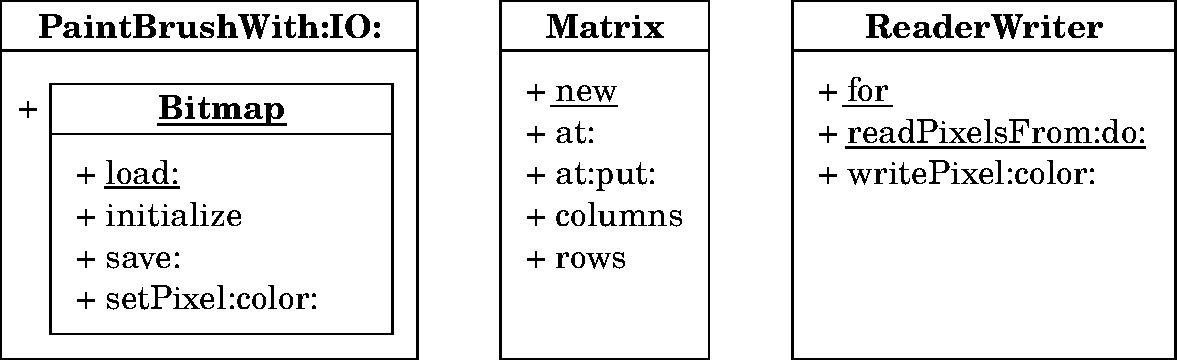
\includegraphics[width=0.8\textwidth]{usecase_paintbrush.pdf}
\caption{Overview of the \texttt{PaintBrushWith:IO:} module and dependent interfaces}
\end{subfigure}

\vspace{10pt}

\begin{subfigure}[b]{\textwidth}
\begin{lstlisting}
<@\textbf{PaintbrushWith:}@> Matrix <@\textbf{IO:}@> ReaderWriter
    <@\textcolor{OliveGreen}{\textbf{< class >}}@>
    ^ Object subclass

<@\textbf{(PaintbrushWith:}@> Matrix <@\textbf{IO:}@> ReaderWriter<@\textbf{) class>>Bitmap}@>
    <@\textcolor{OliveGreen}{\textbf{< class >}}@>
    ^ Object subclassWithInstVars: <@\textcolor{RoyalPurple}{'pixels'}@>

<@\textbf{(PaintbrushWith:}@> Matrix <@\textbf{IO:}@> ReaderWriter<@\textbf{) class>>Bitmap>>initialize}@>
    pixels := Matrix new.

<@\textbf{(PaintbrushWith:}@> Matrix <@\textbf{IO:}@> ReaderWriter<@\textbf{) class>>Bitmap>>}@>
        <@\textbf{setPixel:}@> aPoint <@\textbf{color:}@> aColor
    pixels at: aPoint put: aColor.

<@\textbf{(PaintbrushWith:}@> Matrix <@\textbf{IO:}@> ReaderWriter<@\textbf{) class>>Bitmap class>>}@>
        <@\textbf{load:}@> aFile
    <@\textcolor{Gray}{| instance |}@>
    <@\textcolor{Gray}{instance}@> := self new.
    ReaderWriter 
        readPixelsFrom: aFile
        do: [ :point :color | <@\textcolor{Gray}{instance}@> setPixel: point color: color ].
    ^ <@\textcolor{Gray}{instance}@>

<@\textbf{(PaintbrushWith:}@> Matrix <@\textbf{IO:}@> ReaderWriter<@\textbf{) class>>Bitmap>>save:}@> aFile
    <@\textcolor{Gray}{| writer |}@>
    <@\textcolor{Gray}{writer}@> := ReaderWriter BitmapWriter for: aFile.
    1 to: pixels columns do: [ :x |
        1 to: pixels rows do: [ :y | 
            <@\textcolor{Gray}{writer}@> writePixel: x@y color: (pixels at: x@y) ] ].
    <@\textcolor{Gray}{writer}@> close.
\end{lstlisting}
\caption{Source code for configurable application}
\end{subfigure}
\caption{Parameterized classes for external module configuration}
\label{fig:use_paintbrush}
\end{figure}

It is important to understand that the implementation of \texttt{PaintbrushWith:IO:} is entirely decoupled from the pixel data structure representation and the import/export functionality. It is up to the user of \texttt{PaintbrushWith:IO:} to configure the class as needed.

External configuration as shown in this example is similar to a constructor that accepts class objects as parameters and constructs an instance of the class with the class objects stored in instance variables. The difference to this approach is that, in our system, also class methods are bound to the passed arguments, because a new class object is constructed instead of an instance of a class. Furthermore, our system allows creating new nested classes with the argument as a superclass (mixins).

\section{Hierarchical Decomposition}
\label{sec:usecase_hierach_decomp}
One of the benefits of hierarchical decomposition is better readability and better understandability. Proper class nesting makes it easier for readers of the source code to understand which classes belong together and to find the class containing a certain functionality.

As an example, we took two simple computer games written in Squeak: SpaceCleanup\footnote{\url{https://github.com/matthias-springer/space-cleanup}}, a bomberman clone, and Breakout\footnote{\url{https://github.com/fniephaus/BroBreakout}} (Figure~\ref{fig:usecase_games}).

\begin{figure}[!htp]
\centering
\begin{subfigure}[b]{0.45\textwidth}
    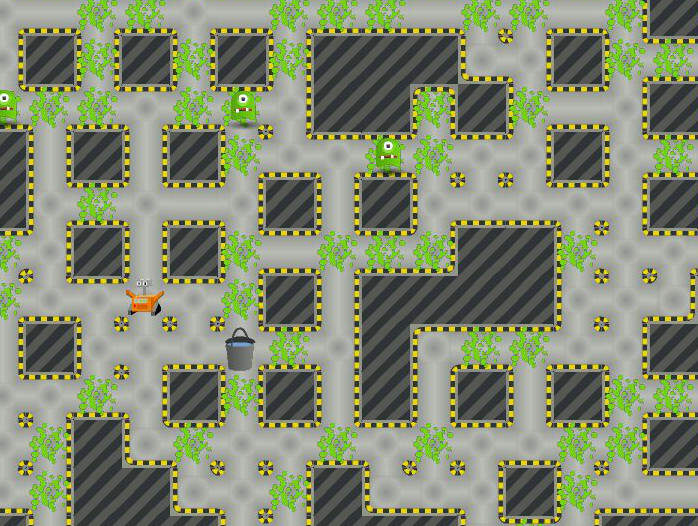
\includegraphics[width=\textwidth]{screen_scleanup.jpeg}
    \caption{SpaceCleanup}
\end{subfigure}
\qquad
\begin{subfigure}[b]{0.45\textwidth}
    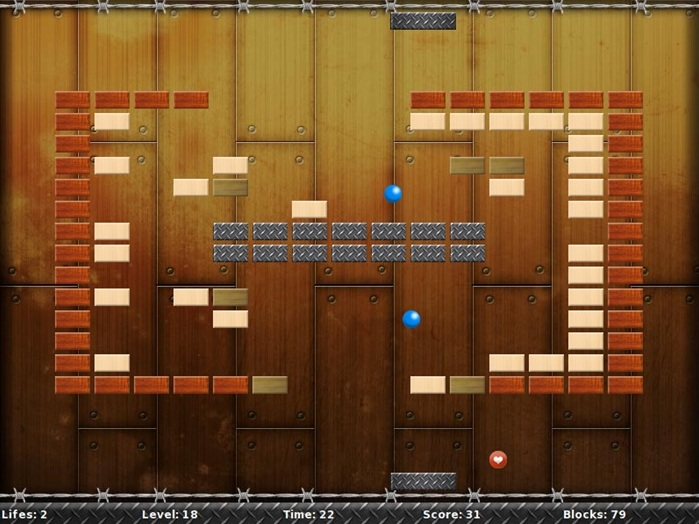
\includegraphics[width=\textwidth]{screen_breakout.jpeg}
    \caption{Breakout}
\end{subfigure}
\caption{Example games as subjects for hierarchical decomposition}
\label{fig:usecase_games}
\end{figure}

Figure~\ref{fig:usecase_sc_space} shows the original source code of SpaceCleanup and the source code after we introduced class nesting. The original source code already made use of packages, which can be compared to a single level of class nesting. The refactored source code is mostly unchanged, except for class name changes. It is interesting to see is that the class structure is already much more readable by just getting rid of all namespace prefixes. We can not only get rid of class prefixes, but also suffixes. For example, \texttt{Builder}, \texttt{Item}, and \texttt{State} suffixes are omitted. It is now also possible to group classes together that belong together logically. For example, both level builders are nested within \texttt{SpaceCleanup Level}. Similarly, all items are nested in \texttt{SpaceCleanup Level Item} (which is also the superclass of all items), which makes sense because a level consists of tiles and every tile can have items. An item cannot be used without a tile and a tile is never used outside a level. Note, that there exist two classes with the name \texttt{Random}, but they are nested in different classes.

\begin{figure}
\begin{subfigure}[b]{0.45\textwidth}
\dirtree{%
.1 \framebox{\textbf{SpaceCleanup}}. 
.2 EventDispatcher.
.2 Level.
.3 \textit{Builder}.
.4 GridPattern.
.4 Random.
.3 Tile.
.4 \textit{Item}.
.5 Bucket.
.5 \textit{Destructible}.
.5 Floor.
.5 Monster.
.6 \textit{Strategy}.
.7 MoveToPlayer.
.7 Random.
.5 \textit{Moving}.
.5 PickUp.
.5 Player.
.5 Portal.
.5 Slime.
.5 Wall.
.5 Water.
.2 \textit{State}.
.3 Building.
.3 Configuring.
.3 GameOver.
.3 GameWon.
.3 Paused.
.3 Running.
.2 Resources.
.2 UI.
.3 CheatWindow.
.3 ConfigurationWindow.
.3 Controls.
.3 GameInformation. 
}
\caption{Refactored project structure}
\end{subfigure}
\qquad
\begin{subfigure}[b]{0.45\textwidth}
\dirtree{%
.1 \framebox{\textbf{SpaceCleanup-Core}}.
.2 ScuEventDispatcher.
.2 ScuGame.
.2 ScuGameBuildState.
.2 ScuGameConfigState.
.2 ScuGameOverState.
.2 ScuGamePausedState.
.2 ScuGameRunningState.
.2 \textit{ScuGameState}.
.2 ScuGameWonState.
.2 \textit{ScuMonsterStrategy}.
.2 ScuMonsterRandomStrategy.
.2 ScuMonsterToPlayerStrategy.
}
\vspace{10pt}
\dirtree{%
.1 \framebox{\textbf{SpaceCleanup-Items}}.
.2 ScuBucket.
.2 \textit{ScuDestructibleItem}.
.2 ScuFloor.
.2 \textit{ScuItem}.
.2 ScuMonster.
.2 \textit{ScuMovingItem}.
.2 ScuPickUpItem.
.2 ScuPlayer.
.2 ScuPortal.
.2 ScuSlime.
.2 ScuWall.
.2 ScuWater.
}
\vspace{10pt}
\dirtree{%
.1 \framebox{\textbf{SpaceCleanup-Level}}.
.2 ScuLevel.
.2 \textit{ScuLevelBuilder}.
.2 ScuGridPatternLevelBuilder.
.2 ScuRandomLevelBuilder.
.2 ScuTile.
}
\vspace{10pt}
\dirtree{%
.1 \framebox{\textbf{SpaceCleanup-Resources}}.
.2 ScuResourceManager.
}
\vspace{10pt}
\dirtree{%
.1 \framebox{\textbf{SpaceCleanup-UI}}.
.2 ScuCheatWindow.
.2 ScuConfigurationWindow.
.2 ScuControls.
.2 ScuGameInformation.
}
\caption{Original project structure}
\label{fig:usecase_sc_origi_fig}
\end{subfigure}
\caption{SpaceCleanup game implementation with/without hierarchical decomposition}
\label{fig:usecase_sc_space}
\end{figure}

Figure~\ref{fig:usecase_breakout_game} shows the original source code of Breakout, as well as a refactored version. We did not change the source code, except for class names. All block-related classes are stored as nested classes in the class \texttt{Breakout Block}, which is also used to represent regular blocks in the game, that can be destroyed using \texttt{Racket}. \texttt{Breakout Block Boundary} represents a special block used for the undestroyable border of the game. All power ups are represented as nested classes in the abstract superclass \texttt{Breakout Powerup}. The structure of the refactored version is much clearer, because the original version did not take advantage of packages, probably due to the relatively small number of classes.

\begin{figure}[!htp]
\begin{subfigure}[b]{0.45\textwidth}
\dirtree{%
.1 \framebox{\textbf{Breakout}}.
.2 Level.
.3 Ball.
.3 Block.
.4 Boundary.
.4 Explosion.
.4 Racket.
.3 Builder.
.3 \textit{Powerup}.
.4 Accelerate.
.4 Ball.
.4 Decelerate.
.4 Enlarge.
.4 Shrink.
.3 World.
.2 \textit{View}.
.3 Level.
.3 Menu.
.3 Welcome.
.2 LevelStatistics.
.3 Item.
.2 MenuLabel.
}
\caption{Refactored project structure}
\end{subfigure}
\qquad
\begin{subfigure}[b]{0.45\textwidth}
\dirtree{%
.1 \framebox{\textbf{BroBreakout}}.
.2 BroBall.
.2 BroBlock.
.2 BroBoundary.
.2 BroBreakout.
.2 BroExplosion.
.2 BroLevelBuilder.
.2 BroLevelStatistics.
.2 BroLevelStatisticsItem.
.2 BroLevelView.
.2 BroLevelWorld.
.2 BroMenuLabel.
.2 BroMenuView.
.2 \textit{BroPowerup}.
.2 BroPowerupAccelerate.
.2 BroPowerupBall.
.2 BroPowerupDecelerate.
.2 BroPowerupEnlarge.
.2 BroPowerupShrink.
.2 BroRacket.
.2 \textit{BroView}.
.2 BroWelcomeView.
}
\caption{Original project structure}
\end{subfigure}
\caption{Breakout game implementation with/without hierarchical decomposition}
\label{fig:usecase_breakout_game}
\end{figure}

%example: large project, where parts of the code can now be understood, given that we have hierarchical nesting. could be an example where grouping according to multiple criteria is needed (would result in n x m packages)

\section{Mixin Modularity with Parameterized Classes}
Parameterized classes can be used to build mixins. Mixins are not a special feature of this system: they are an application of \msname and come for free by just having class nesting as described in the previous sections; they are an immediate consequence of parameterized classes. A mixin is a function that takes as an input a class and outputs a subclass with additional behavior~\cite{bracha1992programming, Bettini:2004:CCH:967900.968200}, i.e., it is a class transformator (also called \emph{abstract subclass}~\cite{Bracha:1990:MI:97945.97982}). 

A mixin can be implemented by writing a class generator method with one parameter which is the input class. The method creates a subclass of that input class and returns it. Associated with that parameterized class generator method is a set of instance-side methods and a set of class-side methods. These are the methods that will be added when applying the mixin.

\paragraph{Recursive Mixin Application}
A mixin can make sure another mixin is applied upon its application. This is done by creating a subclass of a mixin application in the class generator method. Consequently, the system first creates a subclass of the base class, adds the methods of the inner mixin, then creates a subclass of the resulting class, and finally adds the methods of the outer mixin.

\paragraph{Example}
Figure~\ref{fig:concept_mixins} shows an example of parameterized classes and how they can be used to build mixins.

\begin{figure}[!htp]
    \centering
    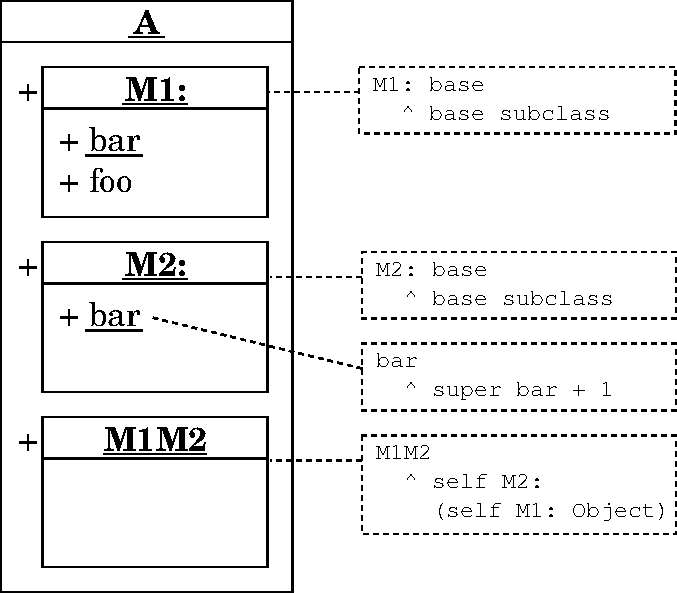
\includegraphics[scale=0.75]{nested_mixins.pdf}
    \caption{Implementation of Mixins with Nested Classes}
    \label{fig:concept_mixins}
\end{figure}

Two class generator methods \texttt{A M1:} and \texttt{A M2:} are defined, which take as input a base class and output a subclass with additional behavior. \texttt{A M1M2} is an application of both both mixins. \texttt{A M1M2}'s superclass is \emph{some} \texttt{A M2:}, whose superclass is \emph{some} \texttt{A M1:}, whose superclass is \texttt{Object}. Note, that \texttt{A M1:} and \texttt{A M2:} are not specific classes: we use this notation as a name for \emph{some} application of \texttt{A class>>M1:} and \texttt{A class>>M2:}, respectively. Therefore, even if two classes have the same name, they are not necessarily the same class if they names contain a colon.

Note, that evaluating \texttt{A M1: Object} multiple times returns different class objects, since parameterized classes are not cached. However, \texttt{A M1M2} is cached, because it is a unary method. Therefore, calling \texttt{A M1M2} multiple times always returns the same class object.

The notation used in \texttt{A class>>M1M2} can be a bit confusing at first. That method first applies \texttt{A M1:} to \texttt{Object}, and then \texttt{A M2:}; however, in the source code, \texttt{A M2:} appears before \texttt{A M1:}. For readability reasons, and to support more features like pre-include hooks and post-include hooks, we present the Class Generator Pattern in Section~\ref{sec:usecase_classgen}.

\section{Unparameterized Class Generator Pattern}
\label{sec:usecase_classgen}
The syntax used for mixin application has a few shortcomings. For example, the statements \texttt{self A: (self B: Object))} means that mixin \texttt{B:} is applied to \texttt{Object}, and then mixin \texttt{A:} is applied to that result. The problem is that the source code statement does not reflect the order of mixin applications: the statement has to be interpreted from right to left. Another problem is that \texttt{A:} and \texttt{B:} are parameterized classes and parameterized classe cannot be referenced using an implicit \texttt{scope} receiver. Therefore, the programmer always has to write \texttt{scope} explicitly.

Both problems can be solved by wrapping the mixin in an unparameterized class and adding a helper method to \texttt{Class}. We assume that the name of the parameterized nested class is always \texttt{Mixin:}. Then, the helper method \texttt{<<} can be defined as shown in Figure~\ref{fig:usecase_class_lele}.

\begin{figure}[!htp]
\begin{lstlisting}
<@\textbf{Class>><< aMixin}@>
    ^ aMixin Mixin: self
\end{lstlisting}
\caption{Helper method on \texttt{Class} for unparameterized mixin wrapper classes}
\label{fig:usecase_class_lele}
\end{figure}

\paragraph{Example}
Figure~\ref{fig:usecase_unparam_class_gen} shows two mixins and a base class: \texttt{CollectionLogic} is a mixin that adds the methods \texttt{allSatisfy:} and \texttt{anySatisfy:}, and \texttt{CollectionFilter} is a mixin that adds the methods \texttt{detect:} and \texttt{select:}. All of these four methods can be implemented based on \texttt{do:}, which iterates through all elements of a collection. Both mixins can be applied to classes providing at least that method. %Consequently, these four methods are written in such a way, meaning that both mixins can be applied classes providing at lease this method.

\begin{figure}[!htp]
\begin{subfigure}[b]{\textwidth}
	\centering
	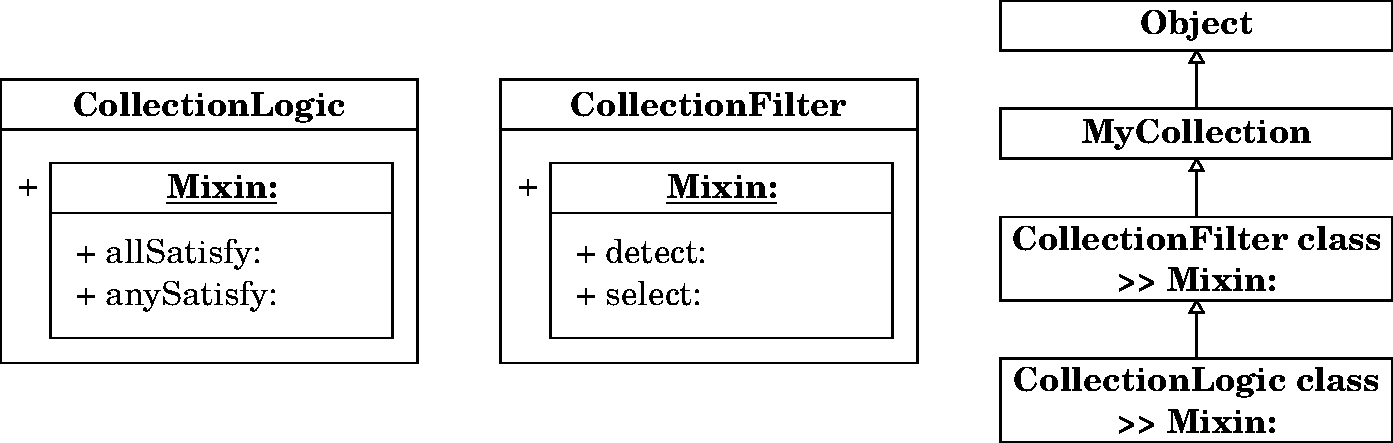
\includegraphics[width=0.95\textwidth]{usecase_classgen.pdf}
	\caption{Class diagram showing mixin and result of mixin application}
\end{subfigure}

\vspace{10pt}

\begin{subfigure}[b]{\textwidth}
\begin{lstlisting}
<@\textbf{CollectionLogic class>>Mixin:}@> base
    <@\textcolor{OliveGreen}{\textbf{< class >}}@>
    ^ base subclass

<@\textbf{(CollectionLogic class>>Mixin:}@> base<@\textbf{)>>allSatisfy:}@> aBlock
    self do: [ :each | 
        (aBlock value: each) ifFalse: [ ^ false ] ].
    ^ true

<@\textbf{(CollectionLogic class>>Mixin:}@> base<@\textbf{)>>anySatisfy:}@> aBlock
    self do: [ :each | 
        (aBlock value: each) ifTrue: [ ^ true ] ].
    ^ false

" (implementation of CollectionLogic omitted) "

<@\textbf{MyCollection>>do:}@> aBlock
    " Some implementation "

<@\textbf{FullCollection}@>
    <@\textcolor{OliveGreen}{\textbf{< class >}}@>
    ^ MyCollection << CollectionFilter << CollectionLogic
\end{lstlisting}
\caption{Definition and application of mixins}
\end{subfigure}
\caption{Unparameterized class generator pattern}
\label{fig:usecase_unparam_class_gen}
\end{figure}

\texttt{CollectionLogic} and \texttt{CollectionFilter} are wrappers around mixins, making it possible to access them like any unparameterized class. When a mixin is applied using the \texttt{<<} syntax, the receiver is used as an argument for the \texttt{Mixin:} method. Therefore, the name of the actual mixin must always be \texttt{Mixin:}, as long as, \texttt{<<} is implemented as shown in Figure~\ref{fig:usecase_class_lele}. Note, that \texttt{<<} inverses the order of receiver and argument, which is why the statement in \texttt{FullCollection} can be read from left to right: first \texttt{CollectionFilter} and then \texttt{CollectionLogic} is applied to \texttt{MyCollection}.

\paragraph{Pre-Include Hooks and Post-Include Hooks}
The unparameterized class generator pattern allows the definition of pre-include hooks and post-include hooks. A pre-include hook is a method defined on the mixin wrapper, which is executed before the mixin was applied, with the base class as an argument. Similarly, a post-include hook is executed after the mixin was applied, with the resulting class as an argument. 

Note, that the programmer can already write arbitrary code at the point where the mixin is applied. However, pre-include hooks and post-include hooks are provided by the mixin itself, and not by the user of a mixin.

\begin{figure}[!htp]
\centering
\begin{subfigure}[b]{0.45\textwidth}
\begin{lstlisting}
<@\textbf{Class>><< aMixin}@>
    <@\textcolor{Gray}{| result |}@>
    aMixin before: self.
    <@\textcolor{Gray}{result}@> := aMixin Mixin: self.
    aMixin after: <@\textcolor{Gray}{result}@>.
    ^ <@\textcolor{Gray}{result}@>
\end{lstlisting}
\caption{Mixin wrapper application}
\end{subfigure}
\qquad
\begin{subfigure}[b]{0.45\textwidth}
	\centering
	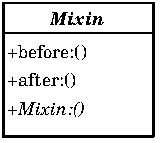
\includegraphics[scale=1]{abstract_mixin_classgen.pdf}
	\caption{Mixin wrapper base class}
\end{subfigure}
\caption{Implementation of pre-incude hooks and post-include hooks for mixins}
\label{fig:usecase_prepostincl}
\end{figure}

Figure~\ref{fig:usecase_prepostincl} shows how these hooks are implemented. Mixins with a pre-include hook or a post-include hook should be a subclass of the abstract class \texttt{Mixin}. This class provides empty \texttt{before:} and \texttt{after:} methods which should be overridden in subclasses and contain the pre-include hook and/or post-include hook.

In the previous paragraph, the unparameterized class generator pattern was presented as a tool to increase code readability. With regards to include hooks, this pattern is more: it is necessary to have some kind of wrapping. Include hooks should not be defined on the mixin function itself, because all methods defined on the mixin function are added during mixin application. This is usually not desirable.

\section{Mixins as Composable Pieces of Behavior}
Mixins, as described in the last two sections, are class transformators. Given an existing class, they output a new subclass with additional or changed behavior. In Figure~\ref{fig:usecase_unparam_class_gen}, we started with \texttt{MyCollection}, a class containing only the \texttt{do:} method, and added additional behavior to it, resulting in the class \texttt{FullCollection}. 

Here is another point of view on the same situation: combine behavior from \texttt{CollectionFilter} and \texttt{CollectionLogic}, add an implementation of \texttt{do:}, and call it \texttt{FullCollection} (Figure~\ref{fig:mixin_composable}).

\begin{figure}[!htp]
\centering
\begin{subfigure}[b]{0.6\textwidth}
\begin{lstlisting}
<@\textbf{FullCollection}@>
    <@\textcolor{OliveGreen}{\textbf{< class >}}@>
    ^ (Object 
        << CollectionFilter 
        << CollectionLogic) subclass

<@\textbf{FullCollection>>do:}@> aBlock
    " Some implementation "
\end{lstlisting}
\end{subfigure}
\qquad
\begin{subfigure}[b]{0.25\textwidth}
    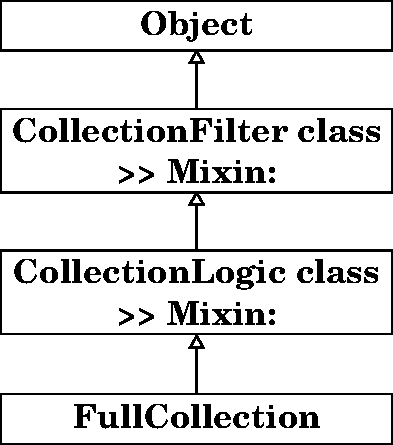
\includegraphics[width=\textwidth]{usecase_classgen_v2.pdf}
\end{subfigure}
\caption{Mixins as composable pieces of behavior}
\label{fig:mixin_composable}
\end{figure}

For readability reasons, our implementation provides a simplified notation that combines this kind of mixin application and subclassing (Figure~\ref{fig:usecase_subcl_mixin}). This new notation first applies mixins, and creates a subclass of the result afterwards. Note, that the notation reflects the order of subclassing: at first, \texttt{Mixin1} is applied, then \texttt{Mixin2}, then \texttt{Mixin3}, and finally a subclass is created with the additional methods defined on \texttt{NewClass}.

\begin{figure}[!htp]
\begin{subfigure}[b]{0.45\textwidth}
\begin{lstlisting}
<@\textbf{NewClass}@>
    <@\textcolor{OliveGreen}{\textbf{< class >}}@>
    ^ Object
        mixin: Mixin1
        mixin: Mixin2
        mixin: Mixin3
        subclassWithInstVars: <@\textcolor{RoyalPurple}{'foo bar'}@>
        classVars: <@\textcolor{RoyalPurple}{'Bar'}@>
        classInstVars: <@\textcolor{RoyalPurple}{'Foo'}@>
\end{lstlisting}
\caption{Mixin and subclass template}
\end{subfigure}
\qquad
\begin{subfigure}[b]{0.45\textwidth}
\begin{lstlisting}
<@\textbf{FullCollection}@>
    <@\textcolor{OliveGreen}{\textbf{< class >}}@>
    ^ Object
        mixin: CollectionFilter
        mixin: CollectionLogic
        subclassWithInstVars: <@\textcolor{RoyalPurple}{''}@>
\end{lstlisting}
\caption{Mixin and subclass example}
\end{subfigure}
\caption{Simplified notation for using subclassing and mixins}
\label{fig:usecase_subcl_mixin}
\end{figure}

The idea of mixins used as composable units of behavior is similar to traits~\cite{traitsschaerli}. However, there are some minor differences.
\begin{itemize}
    \item Mixins are not flat, but create an inheritance hierarchy. E.g., \texttt{FullCollection superclass} returns an application of \texttt{CollectionLogic class>>Mixin:} and not \texttt{Object}.
    \item No explicit conflict resolution is required. Traits raise an error whenever a method is added multiple times and the conflict is not resolved manually in the resulting class. The last applied mixin, on the other hand, overwrites predefined methods with the same name, and allows calling the original implementation using \texttt{super}.
\end{itemize}


\section{Traits}
Traits are similar to mixins and allow behavior to be shared among multiple classes. They can be implemented with class nesting and parameterized classes. The basic idea is to have a parameterized class for every trait, adding trait methods to the target class, but without subclassing it first. Every trait has a pre-include hook and post-include hook. The pre-include hook creates a set of all selectors for the target class. The post-include hook checks if a method was overwritten when it was applied by comparing the set of selectors with the selectors provided by the inner parameterized class. If that is the case, the trait replaces that method with a method that throws an error message, telling the programmer that the conflict has to be resolved. The method provided by the trait is aliased with a selector containing the trait name. In a resolved method (which overwrites the method that throws the conflict error), the programmer can call aliased trait methods.

The idea of traits is not yet fully fledged out at the moment. This section is meant to give a rough idea of what else could be done with \msname (see Section~\ref{sec:app_traits} for details). The described approach still has a few shortcomings.
\begin{itemize}
    \item Conflicts errors are thrown when the resolved method is called and not during trait application.
    \item Adding new methods to Traits that were already applied can break these applications. Every trait is essentially a class extension and adding a new method will add the method to all trait applications, whether or not the method already exists (no conflict resolution).
\end{itemize}

\section{Extension Methods}
\label{sec:usecases_ext_meth}
There are cases, in which the functionality of an already existing class in a different module must be extended or changed. For example, this is the case when a bug in another library must be fixed. The programmer typically writes a method that replaces the existing one with the bug. Sometimes, extension methods are also used add additional behavior. For example, the \texttt{Morphic} package adds the convenience method \texttt{asStringMorph} to \texttt{String}. Sometimes it is sufficient to create a subclass of the class in question, and add the changed behavior only to the subclass. However, there are cases where the application code is not in control of instance creation.

An extension method can be added in \msname by creating a nested class whose class generator method returns an already existing class instead of a new subclass (class extension).

Consider, for example, that we want to add a method \texttt{asString} to the top-level class \texttt{FullCollection} in Figure~\ref{fig:usecase_subcl_mixin}. Figure~\ref{fig:use_ext_meth} shows how to define a method returning the string concatenation of all elements in the collection.

\begin{figure}[!htp]
\begin{lstlisting}
<@\textbf{MyApplication class>>FullCollection}@>
    <@\textcolor{OliveGreen}{\textbf{< class >}}@>
    ^ Repository FullCollection

<@\textbf{MyApplication class>>FullCollection>>asString}@>
    ^ String streamContents: [ :stream |
        self do: [ :each | stream nextPutAll: each asString ] ]
\end{lstlisting}
\caption{Extension methods using nested classes}
\label{fig:use_ext_meth}
\end{figure}

Note, that it is not possible to add extension methods to all parameterized classes or class specifications. Extension methods can only be added to concrete classes (i.e., class objects). For example, it is not possible, to add an extension method to all classes that are generated by \texttt{PaintBrushWith:IO:} in Figure~\ref{fig:use_paintbrush}; only a concrete class object (instantiation) can be extended.

Extension methods are dangerous because changes to existing methods could break other code relying on the old behavior. Numerous alternatives have been proposed, and we provide a brief overview of some of them in Section~\ref{sec:future_ext_meth}.
